\chapter{Mechanischer Aufbau}
\section{Rahmenbedingungen}
Aufgrund des Vorhandenseins eines 3D-Druckers an der Hochschule und der damit verbundenen Flexibilität, haben wir uns entschlossen, das Gehäuse und die Halterungen für die einzelnen Komponenten zu drucken.
Allerdings gilt es auch hierbei einige Dinge zu beachten. Dadurch, dass der Drucker die Modelle schichtenweise von unten nach oben aufbaut, können beispielsweise Löcher in Wänden nur umständlich oder überhaupt nicht realisiert werden. Theoretisch kann dies durch ein Kippen des zu druckenden Körpers oder das Mitdrucken von Hilfselementen umgangen werden. In der Praxis und vor allem dann, wenn solche Probleme auf mehreren Seiten beziehungsweise an sehr filigranen Stellen eines Modells auftreten, nutzen auch diese Methoden nichts mehr.\\
Zudem kann das Innenleben der gedruckten Teile entweder durch eine Art Wabenstruktur oder komplett gefüllt aufgebaut sein. Durch den Aufbau in Form einer Wabenstruktur wird zum einen ein geringerer Verbrauch von Druckmaterialen und zum anderen eine wesentlich geringere Druckzeit erzielt. Vor allem der Zeitfaktor ist dabei nicht unrelevant, da selbst der Druck von einfachen und mittelgroßen Teilen in der Regel mehrere Stunden in Anspruch nimmt. Wenn man jedoch beabsichtigt die Komponenten zu verschrauben, oder ein sehr hohe Stabilität vorsieht, sollte man auf diese Druckart verzichten und einen gefüllten Druck vorziehen.\\
Um in dem Fall, dass ein Teil unseres Modells beschädigt wird, nicht alles erneut drucken zu müssen, ist das Gesamtmodell modular aufgebaut. Jedes Modul weißt entweder den weiblichen oder den männlichen Teil einer Steckverbindung auf.\\
Außerdem ist der Druckbereich eines 3D-Druckers beschränkt. Bei dem von uns genutzten 3D-Drucker sind wir vor allem auf einer der horizonzalen Achsen eingeschränkt. Der hier zur Verfügung stehende Druckbereich von maximal 21,4cm hat somit die Länge unseres Modells bestimmt.

\section{Motorenführung}
Da wir uns dazu entschlossen haben, jeweils beide Räder auf einer Seite über einen O-Ring miteinander zu verbinden, muss es eine möglichkeit geben, diese ein- und nachspannen zu können. Aus diesem Grund haben wir eine Art Schiene modelliert, in der ein Motor über jeweils eine Schraube mit zwei Muttern an der Vorder- sowie Hinterseite befestigt werden kann.
\begin{wrapfigure}[]{h}[4cm]{10cm}
	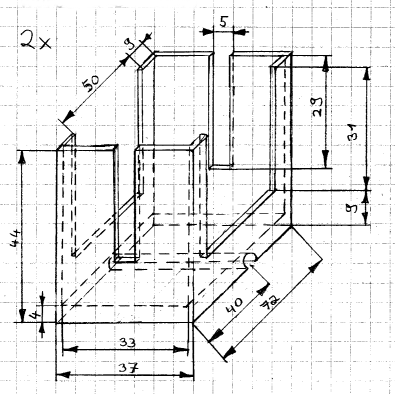
\includegraphics[width=6cm,angle=0]{content/pictures/motorenfuehrung.png}
\end{wrapfigure}
Sie weißt im Inneren eine effektive Länge von 68mm auf und erlaubt es uns somit je nach Größe der Muttern die Motoren mit einer Länge von 40mm um 15mm bis 20mm zu verstellen. Auf der hier gezeigten Skizze ist ein Schraubendurchmesser von 5mm vorgesehen. Dieser kann jedoch beliebig angepasst werden, wenn man die entsprechenden Maße der Motorenführung abändert. Über den weiblichen Teil einer Steckverbindung am unteren Ende wird die Motorenführung später seitlich mit später in der Dokumentation beschriebenen Bodenplatte verbunden.

\section{Motorenfassung}
Die Motoren werden jeweils in einer Halterung eingefasst, welche später in der Motorenführung beweglich gelagert sein wird, um die O-Ringe 
\begin{wrapfigure}[]{h}[4cm]{10cm}
	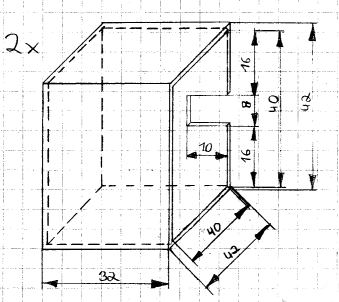
\includegraphics[width=6cm,angle=0]{content/pictures/motorenfassung.png}
\end{wrapfigure}
ein- und nachspannen zu können. Der Primärgrund für die Verwendung solcher Motorenfassungen ist jedoch der, dass die zu den Motoren gehörenden Treiberstufen über ein weiteres Bauteil an den Oberseiten der Motorenfassungen befestigt werden können. Auf diese Weise kann der für die Treiberstufen benötigte Platz auf der Bodenplatte eingespart werden. Zudem ist die Länge der Kabel zwischen Motor und Treiberstufe somit konstant. Um die Kabel, die seitlich aus den Motoren kommen zu berücksichtigen, befindet sich an einer Seite der Motorenfassungen eine entsprechende Aussparung.

